\section{Account} {
    Dopo aver eseguito con successo la registrazione o il login, l'utente avrà accesso alla piattaforma \platform. Da questo momento
    è possibile accedere alla pagina di account, cliccando sulla barra di navigazione il bottone ``\textbf{Account}''. L'utente verrà reindirizzato
    in una nuova pagina contente tale informazioni: 
    \begin{itemize}
        \item Username;
        \item Indirizzo email;
        \item Scelta della visualizzazione della guida;
        \item Lista dei profili seguiti;
        \item Pulsante per il Logout.
    \end{itemize}

    \begin{figure}[H]
        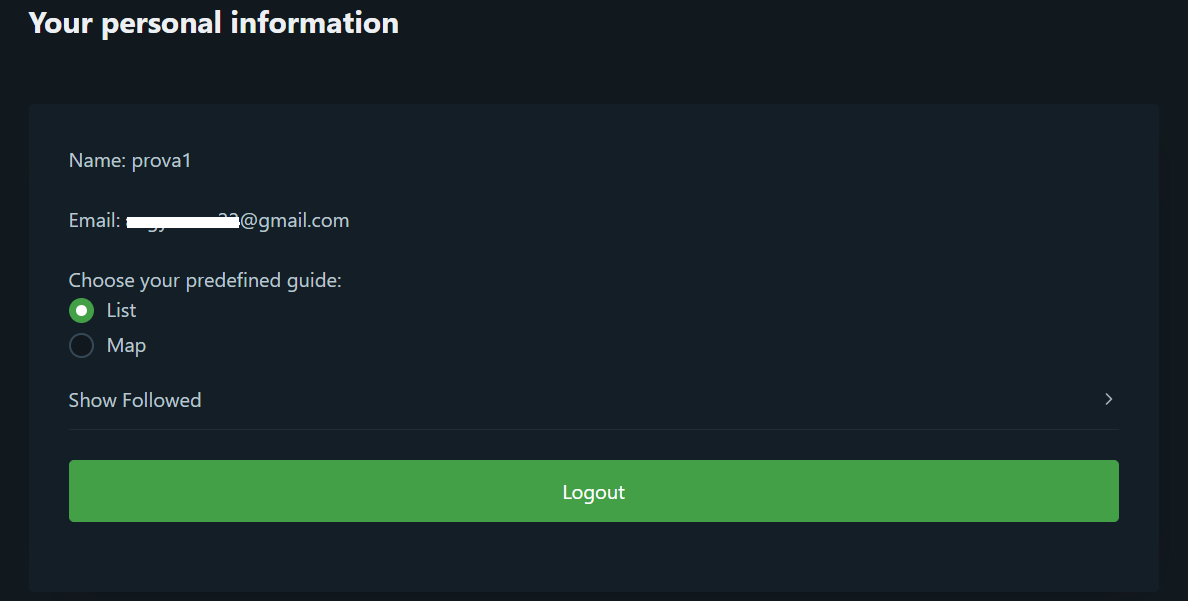
\includegraphics[width=14cm]{sezioni/images/account.png}
        \centering
        \caption{informazioni dell'account personale}
    \end{figure}

    I primi due sono esattamente i campi che si sono compilati nel modulo di registrazione.
    Mentre il pulsante logout è già stato trattato precedentemente. 

    \subsection{Scelta visualizzazione guida} {
        L'utente può decidere la vista predefinita per la visualizzazione della guida nella pagina principale. 
        Le opzioni sono 2: 
        \begin{itemize}
            \item lista: ovvero comparirà una lista di posti;
            \item mappa: i luoghi saranno posizionati all'interno di una mappa con dei segnaposti.
        \end{itemize}
    }


    \subsection{Mostra profili seguiti} {
        L'utente cliccando sull'estensione della tendina visulizzerà una lista dei profili social che segue. 
        Ognuno è caratterizzato da uno username e dal numero di followers (numero di persone della piattaforma \platform{} che seguono tale profilo social). 
        Inoltre è possibile cliccare sul bottone ``\textbf{Rimuovi}'' per smettere di seguire un certo profilo social. 
        \begin{figure}[H]
            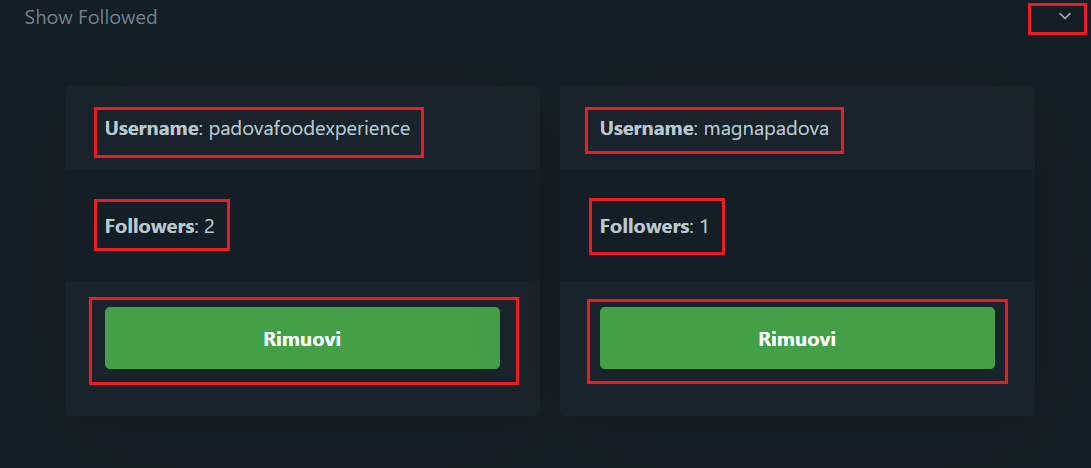
\includegraphics[width=14cm]{sezioni/images/tendina-account.png}
            \centering
            \caption{Tendina per visualizzare e rimuovere i profili social}
        \end{figure}
    }

}
